\documentclass[a4paper,11pt]{extarticle} %este tipo de doc ofrece más tamaños de letra

\usepackage[utf8]{inputenc}%codificación
\usepackage{csquotes}
\usepackage[spanish, mexico]{babel}%Paquete de caracteres y títulos en español de méxico

\usepackage{amsmath, mathtools}%Paquete para insertar símbolos matemáticos
\usepackage{amsbsy}
\usepackage[bitstream-charter]{mathdesign}
\usepackage[mathcal]{eucal}
\DeclareSymbolFont{usualmathcal}{OMS}{cmsy}{m}{n}
\DeclareSymbolFontAlphabet{\mathcal}{usualmathcal}

\usepackage{textcomp}
\usepackage{textcomp,gensymb}

\usepackage[table,xcdraw, dvipsnames]{xcolor}

\usepackage{fontenc}

\usepackage[bottom]{
footmisc}

\usepackage[shortlabels]{enumitem}

\usepackage[tmargin= 2cm,bmargin=2cm,lmargin=2cm,rmargin=2cm]{geometry}

%estos son para tablas y figuras
\usepackage{float}%Paquete para tratar figuras y tablas como flotantes
\usepackage{graphicx}
\graphicspath{ {images/} }
\usepackage{svg}

\usepackage{caption}
\usepackage{subcaption}

\usepackage{physics}

\usepackage{listings}


\usepackage{verbatim}%comentarios en bloque

\captionsetup{font=footnotesize,labelfont=footnotesize} % hace al caption mas chiquito

%convierte los cuadros del caption en tablas
\renewcommand{\listtablename}{Índice de tablas}
\renewcommand{\tablename}{Tabla}

% si quieren usar alfabeto griego sin entrar en mathmode
\usepackage{textgreek}

\usepackage{adjustbox} % para ajustar tablas

\usepackage{url}%Paquete para insertar URL's
\usepackage{hyperref}

\usepackage{multicol}%Paquete para crear ambientes multicolumna
\setlength\columnsep{24pt}%Especifíca separación de las columnas

%este es para la bibliografía yo uso ieee pero se puede cambiar
\usepackage[
backend=biber,
bibencoding=utf8,
style=ieee,
sorting=none
]{biblatex}
\addbibresource{citas.bib}

\usepackage{listings}
\usepackage{xcolor}

% otros nuevos comandos personalizados.
%\newcommand{\dbar} {\ensuremath{\,\mathchar'26\mkern-12mu d}}

 \newcommand
{\cita}[1]{\textsuperscript{\textbf{\cite{#1}}}} % este es para que la cita se vea en superíndice para ieee, si usan otro formato bórrenlo
 \newcommand{\ut}
[1]{\textbf{#1}} %les hace escribir menos si quieren poner negritas en texto y mate
 \newcommand{\um}[1]{\boldsymbol{#1}}
 \renewcommand{\thefootnote}{\Roman{footnote}} %los pie de pagina los pone en letras romanas
 \newcommand{\dbar}{\text{\dj}}
 \newcommand{\parentesis}[1]{\left(#1\right)}
 \newcommand{\crch}[1]{\left[#1\right]}
 
\begin{document}

\begin{center}

	%------------------------------------------------------------------------------------------------------------------------
	% TITULO
	%------------------------------------------------------------------------------------------------------------------------

	\large{\textbf{En búsqueda de la capacitancia del Hilbertrón, un viaje por el método de relajación con ansiedad (diferencias finitas
			centradas de cuarto orden).}}

	\vspace{-\baselineskip}

	\vspace{0.45em}

	%------------------------------------------------------------------------------------------------------------------------
	% INFO CONTACTO
	%------------------------------------------------------------------------------------------------------------------------
	\begin{multicols}{2}
		\begin{center}
			\small{\noindent \textbf {Azpeítia Arias, Ángel Alejandro.}\linebreak
				\noindent \textit{\href{mailto:alejandroazp@ciencias.unam.mx}{alejandroazp@ciencias.unam.mx}}}

		\end{center}
		\columnbreak
		\begin{center}
			\small{\noindent \textbf{ Pérez Flores, Julio Alfonso.}\linebreak
				\noindent \textit{\href{mailto:julio_ perez@ciencias.unam.mx}{julio\textunderscore perez@ciencias.unam.mx}}}

		\end{center}
	\end{multicols}

	\vspace{-\baselineskip}
	\vspace{0.35em}

	\textit{\small{Facultad de Ciencias, Universidad Nacional Autónoma de México. }}

	\small{01 Diciembre, 2023.}

\end{center}

%------------------------------------------------------------------------------------------------------------------------
% RESUMEN
%------------------------------------------------------------------------------------------------------------------------
{\noindent \Large\ut{Resumen.}}

\vspace{0.35em}


\small{Se caracterizo la capacitancia de un condensador coplanar con electrodos basados en seudo curva de Hilbert de segundo orden,
              mediante el método de relajación modificado usando diferencias finitas centradas de cuarto orden, con tolerancia de $2.22 \times 10^{-7}$, además se expone el comportamiento del campo eléctrico, el potencial y la carga. }

\vspace{0.55em}

\textit{\small{\ut{Abstract: The capacitance of a coplanar capacitor with electrodes based on a second-order Hilbert pseudo-curve was characterized using the modified relaxation method employing fourth-order centered finite differences, 
with a tolerance of $2.22 \times 10^{-7}$. Furthermore, the behavior of the electric field, potential, and charge is presented. }}}
\small{ }

\vspace{0.25em}
{\noindent\small{\ut{\textit{Keywords: Space-filling Curve based Electrodes, Coplanar Capacitor, RC Circuit.}}}}

\begin{multicols}{2}
	%------------------------------------------------------------------------------------------------------------------------
	% INTRDODUCCIÓN
	%------------------------------------------------------------------------------------------------------------------------
	\section{Introducción.}

	\subsection{State of Art.}


Un condensador coplanar es un componente electrónico conformado por dos electrodos ubicados en el mismo plano cubiertos por un medio dieléctrico, es importante destacar que la capacitancia de este arreglo tiene atribuciones derivadas de
un campo eléctrico uniforme entre el grosor de los electrodos y otro no uniforme que se dispersa alrededor del espacio en los extremos de los electrodos, conocido como efecto fringe \ut{[bao]} \ut{[eren]}. Cundo un material externo atraviesa este 
ultimo campo eléctrico, la capacitancia asociada es modificada, por lo que esta configuración de electrodos es util para caracterizar cambios en constantes dieléctricas, por el cambio del material o sus propiedades, alguna de los ejemplos 
donde esta aplicación es util es en las técnicas de evaluación no destructivas, la medición de humedad relativa en suelos, y en la detección de fugas de humedad en edificaciones \ut{[mwelango], [cita], [cita]}.  

Abdollahi-Mamoudan et al.\ut{[cita]} muestra que los factores determinantes en la obtención de un valor de capacitancia optimo son la geometría, el espacio entre placas y la frecuencia, cabe destacar que mientras mas área de un electrodos tenga 
frontera con la otra placa, y la separación entre estas sea mas chica, la capacitancia aumenta. Una forma de poder acreditar las condiciones anteriores es mediante el uso de curvas de llenado del espacio [cita] de grosor controlado 
que separen los electrodos. Debido a que la capacitancia se obtiene mediante el desarrollo de la ecuación de Laplace o Poisson, la geometría vuelve a jugar un papel fundamental en la obtención de la capacitancia de forma analítica. Algunas 
geometrías triviales como el de dos tiras coplanares han sido solucionadas mediante el uso de integrales de Cauchy \ut{[zypman]}, algunas geometrías más complejas como un arreglo de anillos han sido solucionadas mediante el uso de la transformada
de Hankel \ut{[guo]}, no obstante; Parker, Naghed y Wolff, [\ut{cita}] y Campbell [\ut{cita}] han mostrado que este problema es soluble mediante método de diferencias finitas.

Es por esto que este trabajo se propone la caracterización de la capacitancia de una geometría basada en una pseudo-curva de Hilbert de segundo orden, mediante el método de relajación \ut{[cita]}, modificandoló de tal forma que se utilices diferencias 
finitas centradas de cuarto orden. Esto con la finalidad de obtener resoluciones a la ecuación de Laplace y al campo eléctrico de geometrías complejas, así como realizar una discusión de la viabilidad de este método para la obtención teórica de
condensadores para la medición de humedad relativa en suelos. 



\subsection{Marco Teórico.}


Para obtener la capacitancia, se necesita calcular la carga en el dispositivo. Se sabe que las cargas eléctricas generan campos eléctricos y magnéticos, que cumplen las cuatro ecuaciones de Maxwell, una de ellas es la ley de Gauss.


\begin{equation}
    \nabla \cdot \Vec{E} =\frac{\rho_{total}}{\epsilon_0}
\end{equation}

Además, para el caso electrostático (las cargas no se mueven), se cumple la igualdad  $\Vec{E}=-\nabla\phi$, remplazando el campo eléctrico en la ley de Gauss se obtiene \ref{poisson} 


\begin{equation}
     \label{poisson}
    \nabla^2 \phi =\frac{-\rho_{total}}{\epsilon_0}
\end{equation}
Y en una región del espacio donde no hay carga eléctrica, se llega a la ecuación  que es nombrada como ecuación de Laplace \ref{laplace}

\begin{equation}
\label{laplace}
    \nabla^2 \phi =0
\end{equation}

Se sabe que por el teorema de existencia y unicidad, que la solución a una ecuación diferencial es única, por lo tanto si encontramos una solución que cumpla las condiciones de frontera es la única solución al problema. 

\begin{equation}
\label{partials}
\nabla^2 \phi = \frac{\partial^2 \phi}{\partial y^2} + \frac{\partial^2 \phi}{\partial x^2} 
\end{equation}




\end{multicols}


\begin{equation}
	\label{aproxV}
	\resizebox{.9\columnwidth }{!}{
		${ \textstyle \phi(x,y)\ \approx\ } {\displaystyle \frac{16 \phi(x - 1,y) + 16 \phi(x,y - 1) + 16 \phi(x + 1,y) + 16 \phi(x,y + 1)
						- \phi(x - 2,y) -  \phi(x,y - 2) - \phi(x + 2,y) - \phi(x,y + 2)}{60}}$
	}
\end{equation}

{\fontsize{8}{7}\selectfont Ecuación \ref{aproxV}: Aproximación del Laplaciano mediante diferencias finitas centradas de cuarto orden. }

\vspace{\baselineskip}

\begin{equation}
	\label{carga}
    \resizebox{.9\columnwidth }{!}{
		${\displaystyle -\frac{\rho(x,y)}{\epsilon_0} \approx\ \frac{16 \phi(x - 1,y) + 16 \phi(x,y - 1) + 16 \phi(x + 1,y) + 16 \phi(x,y + 1)
        - \phi(x - 2,y) -  \phi(x,y - 2) - \phi(x + 2,y) - \phi(x,y + 2)\ - 60\phi(x,y)}{12h^{2}}}$
    }
\end{equation}

{\fontsize{8}{7}\selectfont Ecuación \ref{carga}: Aproximación de la ecuación de Poisson, mediante diferencias finitas centradas de cuarto orden.}



\begin{multicols}{2}
	%%\begin{equation}
%%   \nabla^2 \phi(x,z) \approx \frac{\phi(x+h,z)+\phi(x-h,z)+\phi(x,z+h)+\phi(x,z-h)-4\phi(x,z)}{h^2}
%%\end{equation} 



La ecuación de Laplace puede ser aproximada por el método de relajación, que consiste en aproximar las segundas derivadas parciales por método de diferencias centrales de cuarto orden, como se muestra en la ecuación \ref{dfcco} y \ref{dfcco1}, análogamente para $y$. En la ecuacion \ref{partials} se sustituyen las derivadas centradas, por \ref{laplace} se igual a 0, despejando $\phi(x,y)$, se encuentra que  el valor de cada celda del mallado se aproxima con el promedio de sus cuatro vecinos además haciendo $h=1$ se obtiene \ref{aproxV}.

\begin{equation}
\label{dfcco1}
\resizebox{.9\columnwidth }{!}{
$\dv[2]{\phi}{x} \approx \frac{-\phi_{i+2}\ +\ 16\phi_{i+1}\ -\ 30\phi_{i}\ +\ 16\phi_{i-1} -\phi_{i-2} }{12h^{2}} $
}
\end{equation}
\begin{equation}
\label{dfcco}
\resizebox{.9\columnwidth }{!}{
$\dv[2]{\phi}{y} \approx \frac{-\phi_{j+2}\ +\ 16\phi_{j+1}\ -\ 30\phi_{j}\ +\ 16\phi_{j-1} -\phi_{j-2} }{12h^{2}} $
}
\end{equation}

\noindent \small{donde $i+k\ =\ x_{i}+kh,\ j+k\ =\ x_{j}+kh $, con $x_{i}, x_{j}$ puntos  iniciales} 

\vspace{\baselineskip}


Para calcular el campo eléctrico (por completes), se usa el método de diferencias centrales en cada componente del campo eléctrico partiendo de $\vec{E}=-\nabla \phi$

\begin{equation}
\label{E}
\resizebox{.9\columnwidth }{!}{
$\vec{E} \approx \left( -\frac{\phi(x+h,y)-\phi(x-h,y)}{2h},-\frac{\phi(x,y+h)-\phi(x,y-h)}{2h}\right) $
}
\end{equation}



Como ya se tiene calculado el potencial en toda el área y sabiendo que la ecuación \ref{poisson} se cumple en toda región del espacio, nuevamente podemos aplicar diferencias finitas y llegar a la expresión \ref{carga}

\begin{comment}
   \begin{equation}
\label{carga}
 -\frac{\rho(x,y)}{\epsilon_0} \approx \frac{\phi(x+h,y)+\phi(x-h,z)+\phi(x,y+h)+\phi(x,y-h)-4\phi(x,y)}{h^2}
\end{equation}  
\end{comment}

La capacitancia se define como $C=\frac{Q}{\Delta \phi}$, para calcular la carga total. Donde Q es la carga positiva, pues si la aproximación es buena, tendremos la misma cantidad de carga positiva y negativa. 

\begin{equation}
    \label{cargatotal}
    Q = \int \rho(x,y) dxdy \approx \sum_i \sum_j \rho(i,j) 
\end{equation}
	%------------------------------------------------------------------------------------------------------------------------
	% MÉTODO
	%------------------------------------------------------------------------------------------------------------------------
	\section{Método.}

	Calcularemos la capacitancia del condensador cooplanar con la forma mostrada en la \ref{fig:capacitor}, cuyas dimensiones reales son  $2046 \mu m$ de alto y  $2430 \mu m$ de largo (las dimensiones detalladas se muestran en []), Donde la región azul tendrá potencial fijo $\phi_0=0V$, la región roja  $\phi_0=3.5V$ y la región blanca tendrá  $\phi_0=1.6V$ esperando que el metodo converja más rápido. 
\begin{figure}[H]
		\centering
		\includegraphics[width=0.8\columnwidth]{img/problema.png}

		\caption{Esquema fotodiodo PN }
		\label{fig:capacitor}
\end{figure}

Se empleo un mallado de $2046 \times 2430$, en un arreglo matricial donde cada entrada de la matriz representa un área de $ 1 \mu m \times  1 \mu m$. 

Se aplico el método \ref{aproxV} en la región blanca, para observar como se comporta el potencial, con este potencial se calcula el campo eléctrico en toda el área con la ecuación \ref{E}, finalmente con ayuda de \ref{carga} \ y \ref{cargatotal}, mostraremos la distribución de carga y la carga total. 



	%------------------------------------------------------------------------------------------------------------------------
	\section{Resultados y Discución.}

	Al calcular la matriz de potencial con el método de relajación sobre la región blanca se obtiene la gráfica \ref{fig:potencial}. Donde se aprecia que el potencial tiene un cambio menos drástico.

\begin{figure}[H]
\centering
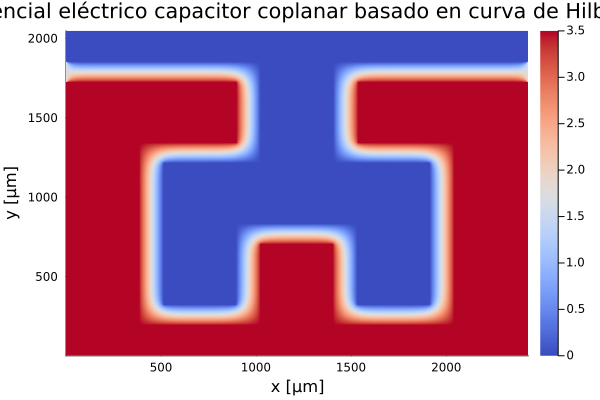
\includegraphics[width=1.1\columnwidth]{img/pothilheat.jpg}
    \caption{Potencial  }
    \label{fig:potencial}
\end{figure}

Para apreciar de mejor manera como cambia el potencial graficámos las lineas equipotenciales donde es claro que siguen el contorno de los electrodos, con suavización en las esquinas, donde hay efectos de borde.  

\begin{figure}[H]
\centering
    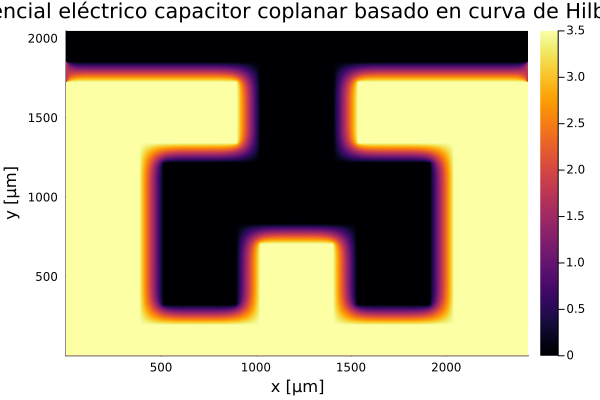
\includegraphics[width=1.2\columnwidth]{img/pothileq.jpg}
    \caption{Lineas equipotenciales  }
    \label{fig:equipV}
\end{figure}

La gráfica del campo eléctrico muestra, lineas son perpendiculares a las lineas equipotenciales, van del cátodo positivo al negativo, lo que indica la precensia de carga positiva y negativa, pues las líneas de campo nacen en las positivas y mueren en las negativas.  


\begin{figure}[H]
\centering
    \includegraphics[width=1.2\columnwidth]{img/Campo.jpg}
    \caption{Campo eléctrico}
    \label{fig:equipV}
\end{figure}

Finalmente al calcular la densidad de carga se obtiene la gráfica, donde podemos apreciar que la carga positiva se acumula en el electrodo con volteje positivo y positiva en el electrodo con voltaje 0.  

\begin{figure}[H]
\centering
    \includegraphics[width=1.2\columnwidth]{}
    \caption{Distribucion de carga}
    \label{fig:equipV}
\end{figure}

Al sumar la carga positiva en se obtiene $Q= 1000 pesos $ y la diferencia de voltaje es 3.5 con lo que la capacitancia es $C=\frac{Q}{\Delta\phi}$

	%------------------------------------------------------------------------------------------------------------------------
	% CONCLUSIONES.
	%------------------------------------------------------------------------------------------------------------------------
	\section{Conclusiones.}

	El método es funcional, para asegurarnos que los resultados son correctos se tendría que hacer la comparación con los resultados experimentales. \\
Otro método que quisimos explorar, era usar la discontinuidad del campo eléctrico, pero como en las esquinas hay picos de potencial, a parece carga acumulada donde no debería haber.\\
Fuera de eso todas las gráficas y resultados coinciden con lo esperado según el electromagnetismo. 

	%------------------------------------------------------------------------------------------------------------------------
	% REFERENCIAS.
	%------------------------------------------------------------------------------------------------------------------------
	\printbibliography[title={Referencias.}]

\end{multicols}


%------------------------------------------------------------------------------------------------------------------------
% APENDICES.
%------------------------------------------------------------------------------------------------------------------------
{\large \textbf{Apéndice A.}}
\input{secciones/apendiceA.tex}
\end{document}




